\section{Theorie}
Eine wichtige Grundlage zum Verständnis vom Ultraschall ist das allgemeine Verhalten von Schall als mechanische Welle 
und ihre Wechselwirkung untereinander. \\ 
Schall wird generell durch seine Frequenz beschrieben, welche von dem Menschen in einem Bereich von $16 \si{\hertz}$ bis $20 \si{\kilo\hertz}$
wahrnehmbar ist. Entsprechend werden durch das untere Ende des Spektrums an höhrbaren Frequenzen tiefe Töne erzeugt,
für hohe Frequenzen folglich hohe Töne. \\
Der Bereich jenseits des Hörbaren (für den Menschen) führt das Spektrum des sogenannten Ultraschall ein. Dieser endet bei 
$1 \si{\giga\hertz} $ und geht von da an in den Hyperschall über. Unterhalb der tiefsten, wahrnehmbaren Töne, also bei $16 \si{\hertz}$
wird von Infraschall gesprochen, charakterisiert durch eben sehr niedriege Frequenzen.

\subsection{Doppler-Effekt}
Treffen nun zwei Schallwellen aufeinander lassen sich verschiedene Effekte feststellen, die insbesondere von zeitlich veränderlichen
Abständen zwischen Quelle und Empfänger abhängen. Unter dieser Bedingung verschiebt sich die gemessene Frequenz für den Empfänger 
propotional zur Änderung der Entfernung. 
Es lassen sich folglich vier verschiedene Fälle finden mit jeweils zwei für eine bewegte Quelle oder eben den Empfänger.
\begin{description}
    \item Bewegte Quelle: \\
    Die Quelle ist in diesem Fall in der Lage sich dem Empfänger zu nähren oder sich zu entfernen, was folglich, durch Verschiebung der Grundfrequenz $f_0$,
    die Wahrnehmung des Empfängers ändert. Bewegt sich also die Quelle mit einer Geschwindigkeit $f$ weg, wird die messbare Frequenz höher $f_{kl}$. Analog wird die Frequenzen
    niedriger $f_{gr}$wenn sich die Quelle auf den Beobachter zubewegt. In der folgenden Formel, mit $c$ als Schallgeschwindigkeit
    \cite{...}, ist der Zusammenhang mathematisch aufgeführt.
\end{description}
\begin{equation}
    \label{eqn:bewegteQuelle}
    f_{kl/gr} = \frac{f_0}{1 \mp \frac{f}{c}}
\end{equation}
\begin{description}
    \item Bewegter Empfänger: \\
    Nach dem Grundsatz, dass wenn die Entfernung der zwei Systeme größer wird auch die vom Empfänger gemessene Frequenz steigt und andersherum,
    folgt für den bewegten Empfänger das gleiche wie für die bewegte Quelle. In diesem Fall sei bei Entfernung von der Quelle weg die gemessene 
    Frequenz als $f_n$ und bei Näherund als $f_h$ bezeichnet. Es folgt die Formel.
\end{description}
\begin{equation}
    \label{eqn:bewegterEmpfaenger}
    f_{h/n} = f_0 \left ( 1 \pm \frac{v}{c} \right )
\end{equation}
Sollten nun beide Frequenzen, die gesendete und die gemessene bekannt sein, liefern die Formeln \eqref{eqn:bewegteQuelle} und \eqref{eqn:bewegterEmpfaenger}
Aufschluss auf die Geschwindigkeit des Bewegten Systems relativ zum Starren. Eine große Anwendung davon findet sich in der 
Geschwindigkeitsmessung von Blutströmen wieder. Hierbei erfährt der Ultraschall eine Frequenzänderung $\Delta f$ im Vergleich zur Grundfrequenz $f_0$,
durch Kontakt mit zum Beispiel schnellen Blutkörpern. 
\begin{equation*}
  \Delta f = f_0 \frac{v}{c} \left ( \text{cos}\alpha + \text{cos}\beta \right )
\end{equation*}
Die hier auftretenden Variablen $\alpha$ und $\beta$ beschreiben den Winkel zwischen dem Geschwindigkeitsvektor des bewegten Objekts
und der Wellennormalen des Schalls. Bei dem hier vorliegenden Impuls-Echo-Verfahren liegen Empfänger und Quelle direkt beieinander, folglich sind 
die Wellennormalen der einfallenden und ausgesendeten Schallwelle parllell. Bis auf ein minus Zeichen unterscheiden sie sich also nicht, was zur Folge hat
\begin{equation*}
    \alpha = \beta,
\end{equation*}
und somit
\begin{equation}
    \label{eqn:deltaf}
    \Delta f = 2 f_0 \frac{v}{c} \text{cos}\alpha.
\end{equation}
Dieser Winkel ändert sich maßgeblich wenn der Schall beispielsweise durch ein Doppler-Prisma mit verstellbaren Winkel $\theta$ eine zusätzliche Brechung erfährt.
Im Prisma selbst $c_p$ \cite{....}, sowie in der Flüssigkeit $c_L$ \cite{....} bewegt sich der Schall  langsamer  was sich mit dem Brechungsgestz verbinden lässt. Dies 
führt anschließend zur vollständigen Bestimmung von $\alpha$ in Awesenheit eines Doppler-Prsima. 
\begin{equation}
    \label{eqn:alphafinal}
    \alpha = 90 \si{\degree} - \text{arcsin} \left( \text{sin}\theta \cdot \frac{c_L}{c_P} \right)
\end{equation}

\begin{figure}
    \centering
    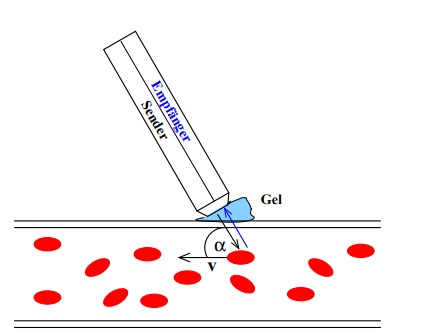
\includegraphics[width=0.5\textwidth]{bilder/winkel.png}
    \caption{Schematische Anwendung des Impuls-Echo-Verfahren auf ein Strömungsprofil. \cite{skript}} 
    \label{fig:figskizze1}
\end{figure}


\subsection{Erzeugung von Ultraschallwellen}
Um Schallwellen im Ultraschallbereich zu Erzeugen bieten sich besonders Piezokristalle an. Diese werden in einem Elektrischen Feld 
zum Schwingen gebracht was im allgemeinen als reziproker piezo-elektrischer Effekt bekannt ist. Wichtig ist das eine Achse des Kristalls
senkrecht auf dem Elektrischen Feld steht, damit es im inneren selbst zu einer Spannung kommt. Bei richtiger Konfiguration werden nun 
Ultraschallwellen gestrahlt bei der besonders die Wellen mit möglichst großer Amplitude von Nutzen sind. 
Dazu wird der Effekt der Resonanz verwendet, welcher auftritt wenn die Anregende Frequenz mit der Eigenfrequenz übereinstimmt.
Dieser Vorgang kann umgekehrt werden. Wenn also ein Piezokristall durch Ultraschall zum Schwingen gebracht wird erzeugt dieser ein messbares
elektrisches Feld welches Aufschluss über die Frequenz der einfallenden Schallwelle gibt. 
Besonders eigenen sich Quarze, die mit ihrer gleichbleibenden physikalischen Eigenschaften, trotz ihrer schwachen erzeugten Amplituden,
eine häufige Anwendung erfahren. 

\begin{figure}
    \centering
    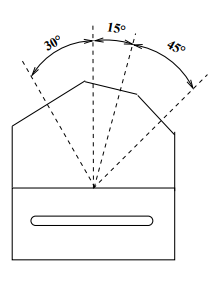
\includegraphics[width=0.5\textwidth]{bilder/winkel2.png}
    \caption{Doppler-Prisma als schematischer Querschnitt mit möglichen Winkelkonfigurationen. \cite{skript}} 
    \label{fig:figskizze1}
\end{figure}